
The design of reward functions constitutes the most consequential architectural decision in any reinforcement learning system, and this principle applies with particular force to the optimization of synthetic data generation parameters for object detection. Unlike traditional reinforcement learning domains where reward signals emerge naturally from environmental dynamics, the synthetic data optimization context requires careful engineering of composite reward functions that integrate detection performance metrics, statistical reliability considerations, and auxiliary signals that promote beneficial exploration behavior. This chapter develops a comprehensive mathematical framework for reward function design, addressing the unique challenges posed by small validation sets, the risk of reward hacking, and the need to balance multiple competing objectives within a coherent optimization framework.

\section{Primary Reward Signals}
\label{sec:primary_reward}

The fundamental objective of synthetic data optimization is to discover generator configurations that produce training corpora yielding detectors with maximal performance on real-world imagery. This objective naturally suggests detection metrics computed on held-out real-world validation sets as the primary reward signal. However, the translation of this intuition into mathematically rigorous reward formulations requires careful consideration of metric properties, aggregation strategies, and the relationship between component metrics and overall detection quality.

\subsection{Mean Average Precision as the Primary Objective}

Mean Average Precision (mAP) has emerged as the predominant evaluation metric for object detection systems, serving as the primary benchmark in competitions such as PASCAL VOC and MS COCO. The metric integrates precision-recall trade-offs across detection thresholds and object classes, providing a comprehensive assessment of detector quality that aligns well with practical deployment requirements.

For a detector producing predictions on a validation set containing ground truth annotations across $C$ object classes, the computation of mAP proceeds through several stages. Let $\mathcal{D} = \{(x_i, \mathcal{Y}_i)\}_{i=1}^{N}$ denote the validation set comprising $N$ images, where each $\mathcal{Y}_i = \{(b_j, c_j)\}_{j=1}^{M_i}$ contains $M_i$ ground truth bounding boxes $b_j \in \mathbb{R}^4$ with associated class labels $c_j \in \{1, \ldots, C\}$. The detector produces predictions $\hat{\mathcal{Y}}_i = \{(\hat{b}_k, \hat{c}_k, \hat{s}_k)\}_{k=1}^{\hat{M}_i}$ where $\hat{s}_k \in [0, 1]$ denotes the confidence score associated with each detection.

The Intersection over Union (IoU) between a predicted bounding box $\hat{b} = (\hat{x}_1, \hat{y}_1, \hat{x}_2, \hat{y}_2)$ and a ground truth box $b = (x_1, y_1, x_2, y_2)$ is computed as:
\begin{equation}
\text{IoU}(\hat{b}, b) = \frac{|\hat{b} \cap b|}{|\hat{b} \cup b|} = \frac{\text{Area}(\hat{b} \cap b)}{\text{Area}(\hat{b}) + \text{Area}(b) - \text{Area}(\hat{b} \cap b)}
\label{eq:iou_definition}
\end{equation}
where the intersection area is computed as:
\begin{equation}
\text{Area}(\hat{b} \cap b) = \max(0, \min(\hat{x}_2, x_2) - \max(\hat{x}_1, x_1)) \cdot \max(0, \min(\hat{y}_2, y_2) - \max(\hat{y}_1, y_1))
\end{equation}

A detection is classified as a true positive for class $c$ at IoU threshold $\tau$ if there exists a ground truth box $b$ of the same class such that $\text{IoU}(\hat{b}, b) \geq \tau$ and neither the prediction nor the ground truth has been previously matched. The matching proceeds in order of decreasing confidence scores $\hat{s}_k$, ensuring that higher-confidence predictions receive priority in the matching process.

Let $\text{TP}_c(\tau, t)$ and $\text{FP}_c(\tau, t)$ denote the cumulative true positive and false positive counts for class $c$ at IoU threshold $\tau$ when considering all predictions with confidence scores exceeding threshold $t$. The precision and recall at this operating point are:
\begin{equation}
P_c(\tau, t) = \frac{\text{TP}_c(\tau, t)}{\text{TP}_c(\tau, t) + \text{FP}_c(\tau, t)}, \quad R_c(\tau, t) = \frac{\text{TP}_c(\tau, t)}{|\mathcal{G}_c|}
\label{eq:precision_recall}
\end{equation}
where $|\mathcal{G}_c|$ denotes the total number of ground truth objects of class $c$ across the validation set.

The precision-recall curve for class $c$ at IoU threshold $\tau$ is obtained by varying the confidence threshold $t$ and computing the corresponding precision-recall pairs. The Average Precision (AP) for class $c$ is computed as the area under this curve:
\begin{equation}
\text{AP}_c(\tau) = \int_0^1 P_c(\tau, R) \, dR \approx \sum_{k=1}^{K} (R_k - R_{k-1}) \cdot P_{\text{interp}}(R_k)
\label{eq:average_precision}
\end{equation}
where $P_{\text{interp}}(R_k) = \max_{R' \geq R_k} P(R')$ represents the interpolated precision at recall level $R_k$, following the eleven-point or all-point interpolation schemes employed in standard benchmarks.

The mean Average Precision across all classes is then:
\begin{equation}
\text{mAP}(\tau) = \frac{1}{C} \sum_{c=1}^{C} \text{AP}_c(\tau)
\label{eq:map_single_threshold}
\end{equation}

The COCO-style mAP extends this computation by averaging across multiple IoU thresholds:
\begin{equation}
\text{mAP}_{\text{COCO}} = \frac{1}{|\mathcal{T}|} \sum_{\tau \in \mathcal{T}} \text{mAP}(\tau)
\label{eq:map_coco}
\end{equation}
where $\mathcal{T} = \{0.50, 0.55, \ldots, 0.95\}$ comprises ten IoU thresholds spanning from lenient to stringent matching criteria.

\begin{figure}[t]
\centering
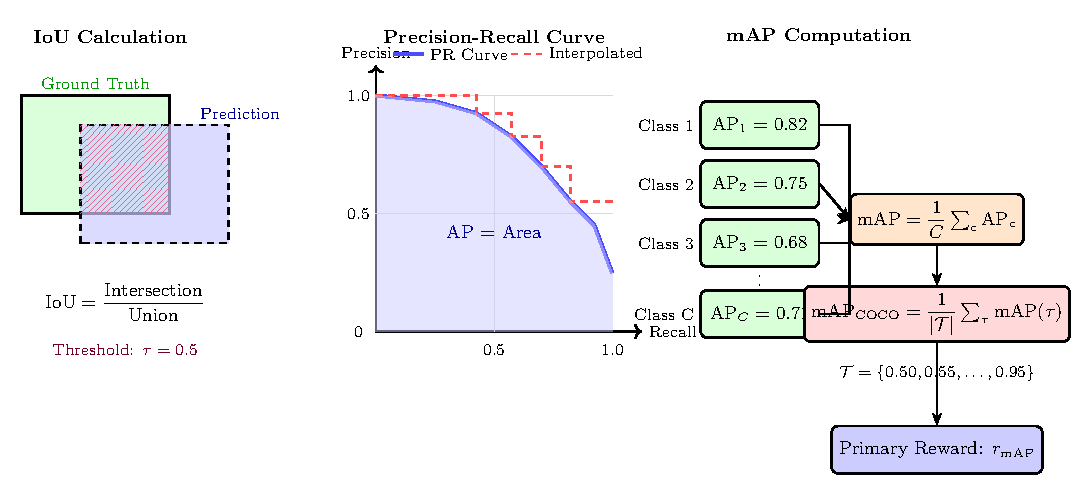
\includegraphics[width=\textwidth]{figures/ch07_fig1_map_calculation.pdf}
\caption{Visualization of mAP computation showing three key stages: (left) IoU calculation between predicted and ground truth bounding boxes with the intersection highlighted, (center) precision-recall curve with the shaded area representing Average Precision, and (right) aggregation of per-class AP values into mAP and the COCO-style averaging across multiple IoU thresholds.}
\label{fig:map_calculation}
\end{figure}

The primary reward signal based on mAP is thus defined as:
\begin{equation}
r_{\text{mAP}} = \text{mAP}_{\text{COCO}}(\theta) = \text{mAP}(\mathcal{D}_{\text{val}}, f_{\phi(\theta)})
\label{eq:reward_map}
\end{equation}
where $\theta$ denotes the synthetic data generator parameters, $\phi(\theta)$ represents the detector weights obtained by training on synthetic data generated with parameters $\theta$, and $f_{\phi(\theta)}$ denotes the resulting detector.

\subsection{Component Metrics and Their Relationships}

While mAP serves as the primary optimization objective, understanding the component metrics provides valuable diagnostic information and enables the construction of more nuanced reward signals. The decomposition of detection performance into precision, recall, and localization quality reveals distinct failure modes that may require targeted intervention through auxiliary reward components.

Precision measures the fraction of detector predictions that correspond to actual objects, quantifying the rate of false positive errors. High precision is essential in applications where false alarms carry significant costs, such as autonomous driving scenarios where phantom detections might trigger unnecessary emergency maneuvers. The precision at a fixed confidence threshold $t^*$ is given by:
\begin{equation}
\text{Precision}(t^*) = \frac{\sum_{c=1}^{C} \text{TP}_c(\tau, t^*)}{\sum_{c=1}^{C} (\text{TP}_c(\tau, t^*) + \text{FP}_c(\tau, t^*))}
\label{eq:precision_fixed}
\end{equation}

Recall measures the fraction of ground truth objects successfully detected, quantifying the rate of false negative errors. High recall is critical in applications where missed detections carry severe consequences, such as medical imaging where overlooked abnormalities might delay life-saving treatment. The recall at confidence threshold $t^*$ is:
\begin{equation}
\text{Recall}(t^*) = \frac{\sum_{c=1}^{C} \text{TP}_c(\tau, t^*)}{\sum_{c=1}^{C} |\mathcal{G}_c|}
\label{eq:recall_fixed}
\end{equation}

The F1 score provides a harmonic mean of precision and recall, offering a single metric that penalizes extreme imbalances between the two:
\begin{equation}
F_1 = \frac{2 \cdot \text{Precision} \cdot \text{Recall}}{\text{Precision} + \text{Recall}} = \frac{2 \cdot \text{TP}}{2 \cdot \text{TP} + \text{FP} + \text{FN}}
\label{eq:f1_score}
\end{equation}

Localization quality, as captured by the IoU distribution of matched detections, provides insight into the geometric accuracy of bounding box predictions. The mean IoU of true positive detections is:
\begin{equation}
\overline{\text{IoU}} = \frac{1}{|\text{TP}|} \sum_{(\hat{b}, b) \in \text{TP}} \text{IoU}(\hat{b}, b)
\label{eq:mean_iou}
\end{equation}

\subsection{Class-Specific versus Aggregate Rewards}

The aggregation strategy employed when combining per-class metrics into a scalar reward has significant implications for optimization dynamics, particularly when class frequencies are imbalanced or when different classes exhibit varying difficulty levels.

The standard mAP formulation employs uniform weighting across classes, treating all classes as equally important regardless of their frequency in the validation set:
\begin{equation}
r_{\text{uniform}} = \frac{1}{C} \sum_{c=1}^{C} \text{AP}_c
\label{eq:uniform_weighting}
\end{equation}

Frequency-weighted aggregation assigns weights proportional to class prevalence, emphasizing performance on common classes:
\begin{equation}
r_{\text{freq}} = \sum_{c=1}^{C} \frac{|\mathcal{G}_c|}{\sum_{c'} |\mathcal{G}_{c'}|} \cdot \text{AP}_c
\label{eq:frequency_weighting}
\end{equation}

Inverse-frequency weighting places greater emphasis on rare classes, which may be appropriate when rare classes carry particular practical importance:
\begin{equation}
r_{\text{inv-freq}} = \sum_{c=1}^{C} \frac{1/|\mathcal{G}_c|}{\sum_{c'} 1/|\mathcal{G}_{c'}|} \cdot \text{AP}_c
\label{eq:inverse_frequency_weighting}
\end{equation}

Worst-case class performance provides a max-min objective that prevents the optimizer from sacrificing performance on difficult classes:
\begin{equation}
r_{\text{worst}} = \min_{c \in \{1, \ldots, C\}} \text{AP}_c
\label{eq:worst_case}
\end{equation}

A hybrid formulation that balances average performance with worst-case guarantees employs a convex combination:
\begin{equation}
r_{\text{hybrid}} = (1 - \lambda) \cdot \text{mAP} + \lambda \cdot \min_c \text{AP}_c
\label{eq:hybrid_aggregation}
\end{equation}
where $\lambda \in [0, 1]$ controls the trade-off between average and worst-case optimization.

\subsection{Confidence-Weighted Metrics}

The confidence scores produced by modern object detectors provide valuable information about prediction reliability that can be incorporated into reward formulations. Confidence-weighted metrics encourage the detector to produce well-calibrated predictions where confidence scores accurately reflect detection accuracy.

The Expected Calibration Error (ECE) measures the discrepancy between predicted confidence and empirical accuracy:
\begin{equation}
\text{ECE} = \sum_{m=1}^{M} \frac{|B_m|}{N} \left| \text{acc}(B_m) - \text{conf}(B_m) \right|
\label{eq:ece}
\end{equation}
where predictions are partitioned into $M$ bins $\{B_m\}$ based on confidence scores, $\text{acc}(B_m)$ denotes the fraction of predictions in bin $B_m$ that are true positives, and $\text{conf}(B_m)$ denotes the average confidence in the bin.

A reward term penalizing miscalibration can be incorporated as:
\begin{equation}
r_{\text{calibration}} = 1 - \text{ECE}
\label{eq:calibration_reward}
\end{equation}

Confidence-weighted precision assigns greater importance to high-confidence predictions:
\begin{equation}
\text{Precision}_{\text{conf}} = \frac{\sum_k \hat{s}_k \cdot \mathbb{1}[\text{TP}_k]}{\sum_k \hat{s}_k}
\label{eq:confidence_weighted_precision}
\end{equation}
where $\mathbb{1}[\text{TP}_k]$ indicates whether prediction $k$ is a true positive.

\section{Handling Small Validation Sets}
\label{sec:small_validation}

The practical constraints of many synthetic data optimization scenarios necessitate validation against severely limited real-world imagery, often comprising fewer than one hundred annotated frames. This limitation introduces substantial statistical challenges, as performance estimates computed on small samples exhibit high variance and may not reliably indicate true detector quality. This section develops mathematical frameworks for addressing these challenges through bootstrap confidence estimation, cross-validation strategies, and variance reduction techniques.

\subsection{Statistical Challenges with Limited Samples}

Consider the task of estimating mAP from a validation set containing $N = 50$ images. The standard error of the mAP estimate depends on the underlying variance of per-image performance and can be approximated as:
\begin{equation}
\text{SE}(\widehat{\text{mAP}}) \approx \frac{\sigma_{\text{mAP}}}{\sqrt{N}}
\label{eq:standard_error}
\end{equation}
where $\sigma_{\text{mAP}}$ represents the standard deviation of per-image AP contributions.

For typical object detection scenarios where $\sigma_{\text{mAP}} \approx 0.15$, a validation set of 50 images yields a standard error of approximately 0.02, implying that 95\% confidence intervals span roughly $\pm 0.04$ mAP points. This level of uncertainty is substantial relative to the performance improvements typically sought through synthetic data optimization, which may target gains of 0.05 to 0.10 mAP points.

The challenge is compounded by the non-uniform distribution of objects across images. Let $n_i$ denote the number of ground truth objects in image $i$. The effective sample size for estimating class-specific AP depends on the total object count rather than the image count:
\begin{equation}
N_{\text{eff},c} = \sum_{i=1}^{N} n_{i,c}
\label{eq:effective_sample_size}
\end{equation}
where $n_{i,c}$ counts objects of class $c$ in image $i$. For rare classes with $N_{\text{eff},c} < 20$, AP estimates become highly unreliable.

\subsection{Bootstrap Confidence Intervals}

Bootstrap resampling provides a non-parametric approach to estimating the sampling distribution of mAP and constructing confidence intervals that account for the complex dependence structure of detection metrics. The procedure involves repeatedly resampling the validation set with replacement and computing mAP on each bootstrap sample.

\begin{algorithm}[t]
\caption{Bootstrap Confidence Interval for mAP}
\label{alg:bootstrap_confidence}
\begin{algorithmic}[1]
\Require Validation set $\mathcal{D} = \{(x_i, \mathcal{Y}_i)\}_{i=1}^{N}$, detector $f$, number of bootstrap samples $B$, confidence level $1 - \alpha$
\Ensure Point estimate $\widehat{\text{mAP}}$, confidence interval $[\text{mAP}_{\text{lo}}, \text{mAP}_{\text{hi}}]$
\State Compute point estimate $\widehat{\text{mAP}} \gets \text{mAP}(\mathcal{D}, f)$
\For{$b = 1$ to $B$}
    \State Sample indices $\mathcal{I}^{(b)} \gets \{i_1^{(b)}, \ldots, i_N^{(b)}\}$ uniformly with replacement from $\{1, \ldots, N\}$
    \State Construct bootstrap sample $\mathcal{D}^{(b)} \gets \{(x_{i_j^{(b)}}, \mathcal{Y}_{i_j^{(b)}})\}_{j=1}^{N}$
    \State Compute bootstrap estimate $\text{mAP}^{(b)} \gets \text{mAP}(\mathcal{D}^{(b)}, f)$
\EndFor
\State Compute bootstrap standard error $\hat{\sigma}_{\text{boot}} \gets \sqrt{\frac{1}{B-1} \sum_{b=1}^{B} (\text{mAP}^{(b)} - \bar{\text{mAP}})^2}$
\State Sort bootstrap estimates: $\text{mAP}^{(1)} \leq \text{mAP}^{(2)} \leq \cdots \leq \text{mAP}^{(B)}$
\State \textbf{Percentile method:} $\text{mAP}_{\text{lo}} \gets \text{mAP}^{(\lfloor B \cdot \alpha/2 \rfloor)}$, $\text{mAP}_{\text{hi}} \gets \text{mAP}^{(\lceil B \cdot (1-\alpha/2) \rceil)}$
\State \textbf{BCa correction (optional):} Apply bias-correction and acceleration adjustments
\State \Return $\widehat{\text{mAP}}$, $[\text{mAP}_{\text{lo}}, \text{mAP}_{\text{hi}}]$
\end{algorithmic}
\end{algorithm}

The percentile bootstrap confidence interval is obtained by taking the $\alpha/2$ and $1 - \alpha/2$ quantiles of the bootstrap distribution. For a 95\% confidence interval with $B = 1000$ bootstrap samples, this corresponds to the 25th and 975th order statistics.

The bias-corrected and accelerated (BCa) bootstrap provides improved coverage properties by adjusting for bias and skewness in the bootstrap distribution:
\begin{equation}
\text{mAP}_{\text{lo}}^{\text{BCa}} = \hat{G}^{-1}\left( \Phi\left( \hat{z}_0 + \frac{\hat{z}_0 + z_{\alpha/2}}{1 - \hat{a}(\hat{z}_0 + z_{\alpha/2})} \right) \right)
\label{eq:bca_lower}
\end{equation}
where $\hat{G}$ denotes the empirical CDF of bootstrap estimates, $\Phi$ is the standard normal CDF, $z_{\alpha/2} = \Phi^{-1}(\alpha/2)$, and the bias-correction factor $\hat{z}_0$ and acceleration factor $\hat{a}$ are computed from the bootstrap distribution and jackknife influence values, respectively.

The bias-correction factor is estimated as:
\begin{equation}
\hat{z}_0 = \Phi^{-1}\left( \frac{1}{B} \sum_{b=1}^{B} \mathbb{1}[\text{mAP}^{(b)} < \widehat{\text{mAP}}] \right)
\label{eq:bias_correction}
\end{equation}

The acceleration factor is computed using jackknife resampling:
\begin{equation}
\hat{a} = \frac{\sum_{i=1}^{N} (\bar{\theta}_{(\cdot)} - \hat{\theta}_{(-i)})^3}{6 \left( \sum_{i=1}^{N} (\bar{\theta}_{(\cdot)} - \hat{\theta}_{(-i)})^2 \right)^{3/2}}
\label{eq:acceleration_factor}
\end{equation}
where $\hat{\theta}_{(-i)}$ denotes the mAP estimate with the $i$-th image removed and $\bar{\theta}_{(\cdot)} = \frac{1}{N} \sum_i \hat{\theta}_{(-i)}$.

\subsection{Cross-Validation Strategies}

Cross-validation provides an alternative approach to variance reduction that partitions the validation set into complementary subsets, enabling more robust performance estimation through averaging across multiple evaluation folds.

$K$-fold cross-validation partitions the validation set into $K$ disjoint subsets $\{\mathcal{D}_1, \ldots, \mathcal{D}_K\}$ and computes performance on each fold:
\begin{equation}
\widehat{\text{mAP}}_{\text{CV}} = \frac{1}{K} \sum_{k=1}^{K} \text{mAP}(\mathcal{D}_k, f)
\label{eq:cv_estimate}
\end{equation}

The variance of the cross-validation estimate can be approximated as:
\begin{equation}
\text{Var}(\widehat{\text{mAP}}_{\text{CV}}) \approx \frac{\sigma^2_{\text{fold}}}{K} + \frac{K-1}{K} \rho \sigma^2_{\text{fold}}
\label{eq:cv_variance}
\end{equation}
where $\sigma^2_{\text{fold}}$ is the variance of per-fold estimates and $\rho$ is the correlation between estimates computed on different folds. The second term reflects the positive correlation induced by shared training data (when cross-validation is applied to the training procedure) or shared model parameters (when applied only to evaluation).

Stratified cross-validation ensures that each fold maintains approximately the same class distribution as the full validation set, which is particularly important when class frequencies are imbalanced:
\begin{equation}
\frac{|\mathcal{G}_{c,k}|}{|\mathcal{D}_k|} \approx \frac{|\mathcal{G}_c|}{|\mathcal{D}|} \quad \forall c, k
\label{eq:stratified_cv}
\end{equation}

Repeated cross-validation performs multiple rounds of $K$-fold cross-validation with different random partitions, further reducing variance at the cost of increased computation:
\begin{equation}
\widehat{\text{mAP}}_{\text{RCV}} = \frac{1}{R \cdot K} \sum_{r=1}^{R} \sum_{k=1}^{K} \text{mAP}(\mathcal{D}_{r,k}, f)
\label{eq:repeated_cv}
\end{equation}

\subsection{Variance Reduction Techniques}

Beyond bootstrap and cross-validation, several additional techniques can reduce the variance of reward estimates, improving the signal-to-noise ratio available to the reinforcement learning optimizer.

Control variates exploit correlation with auxiliary variables whose expectations are known. Let $Y = \text{mAP}$ be the quantity of interest and $X$ be a correlated auxiliary variable. The control variate estimator is:
\begin{equation}
\hat{Y}_{\text{CV}} = Y - \beta(X - \mathbb{E}[X])
\label{eq:control_variate}
\end{equation}
where $\beta^* = \text{Cov}(Y, X) / \text{Var}(X)$ minimizes variance. In the synthetic data context, $X$ might represent performance on a larger synthetic validation set, with $\mathbb{E}[X]$ estimated from historical data.

Antithetic variates reduce variance by introducing negative correlation between paired samples. When evaluating multiple generator configurations, antithetic sampling ensures that high-variance images appear in complementary positions across evaluations, inducing negative covariance that reduces the variance of performance differences.

Common random numbers use the same random seed for stochastic elements (such as data augmentation during evaluation) across different generator configurations, ensuring that performance differences reflect true configuration effects rather than random variation:
\begin{equation}
\text{Var}(\hat{Y}_1 - \hat{Y}_2) = \text{Var}(\hat{Y}_1) + \text{Var}(\hat{Y}_2) - 2\text{Cov}(\hat{Y}_1, \hat{Y}_2)
\label{eq:common_random_numbers}
\end{equation}

When evaluations share random elements, $\text{Cov}(\hat{Y}_1, \hat{Y}_2) > 0$, reducing the variance of the difference.

\subsection{Conservative Reward Estimation}

Given the high variance of performance estimates on small validation sets, conservative reward estimation provides a principled approach to avoiding over-optimistic evaluations that might lead to poor generalization. Rather than using the point estimate $\widehat{\text{mAP}}$, conservative approaches employ lower confidence bounds:
\begin{equation}
r_{\text{conservative}} = \widehat{\text{mAP}} - \kappa \cdot \hat{\sigma}_{\text{boot}}
\label{eq:conservative_reward}
\end{equation}
where $\kappa > 0$ controls the degree of conservatism. Setting $\kappa = 1.96$ corresponds to using the lower bound of a 95\% confidence interval.

The lower confidence bound (LCB) approach is analogous to acquisition functions in Bayesian optimization and implements a form of pessimism under uncertainty that has theoretical justification in the bandit literature. By penalizing high-variance configurations, LCB encourages exploration of regions where performance estimates are reliable.

\section{Reward Shaping Strategies}
\label{sec:reward_shaping}

Pure reliance on the terminal mAP signal presents several challenges for reinforcement learning optimization. The reward is sparse, available only after complete detector training cycles that may require hours of computation. The signal is noisy due to small validation set sizes. And the reward provides limited guidance about the direction of improvement, offering only a scalar summary of detector quality without indicating which aspects of synthetic data generation require modification. Reward shaping addresses these limitations by introducing intermediate signals that guide learning while preserving the optimality of policies that maximize the original objective.

\subsection{Intermediate Rewards During Training}

The detector training process generates a rich stream of intermediate signals that can inform reward computation without waiting for final convergence. Training loss curves, validation performance trajectories, and convergence dynamics all provide information about the quality of synthetic data that can be incorporated into shaped reward functions.

The training loss at epoch $e$ when training on synthetic data generated with parameters $\theta$ is denoted $\mathcal{L}_{\text{train}}(e; \theta)$. The rate of loss decrease provides a signal about learning efficiency:
\begin{equation}
\Delta \mathcal{L}(e; \theta) = \mathcal{L}_{\text{train}}(e-1; \theta) - \mathcal{L}_{\text{train}}(e; \theta)
\label{eq:loss_decrease}
\end{equation}

Configurations yielding faster initial loss decrease often indicate better alignment between synthetic and real data distributions, as the detector can more readily extract transferable features.

An intermediate reward based on early training dynamics is:
\begin{equation}
r_{\text{early}}(\theta) = \frac{1}{E_{\text{early}}} \sum_{e=1}^{E_{\text{early}}} \Delta \mathcal{L}(e; \theta)
\label{eq:early_training_reward}
\end{equation}
where $E_{\text{early}} \ll E_{\text{total}}$ represents an early checkpoint (e.g., 10\% of total training epochs).

The validation loss trajectory provides complementary information about generalization:
\begin{equation}
r_{\text{val-trajectory}}(\theta) = -\min_{e \leq E_{\text{total}}} \mathcal{L}_{\text{val}}(e; \theta)
\label{eq:val_trajectory_reward}
\end{equation}

\subsection{Loss-Based Progress Signals}

The components of the YOLO loss function provide granular feedback about different aspects of detector learning. The total loss decomposes as:
\begin{equation}
\mathcal{L}_{\text{YOLO}} = \lambda_{\text{box}} \mathcal{L}_{\text{box}} + \lambda_{\text{obj}} \mathcal{L}_{\text{obj}} + \lambda_{\text{cls}} \mathcal{L}_{\text{cls}}
\label{eq:yolo_loss_decomposition}
\end{equation}
where $\mathcal{L}_{\text{box}}$ measures localization accuracy, $\mathcal{L}_{\text{obj}}$ measures objectness prediction quality, and $\mathcal{L}_{\text{cls}}$ measures classification accuracy.

Modern YOLO variants employ CIoU (Complete Intersection over Union) loss for bounding box regression:
\begin{equation}
\mathcal{L}_{\text{CIoU}} = 1 - \text{IoU} + \frac{\rho^2(b, b^{\text{gt}})}{c^2} + \alpha v
\label{eq:ciou_loss}
\end{equation}
where $\rho(b, b^{\text{gt}})$ is the Euclidean distance between box centers, $c$ is the diagonal length of the smallest enclosing box, $v = \frac{4}{\pi^2}(\arctan(w^{\text{gt}}/h^{\text{gt}}) - \arctan(w/h))^2$ measures aspect ratio consistency, and $\alpha = v / ((1 - \text{IoU}) + v)$.

Monitoring the convergence of individual loss components enables diagnosis of synthetic data deficiencies. Slow convergence of $\mathcal{L}_{\text{box}}$ may indicate unrealistic object scales or positions in synthetic data. Poor $\mathcal{L}_{\text{cls}}$ convergence suggests insufficient class-discriminative features. Elevated $\mathcal{L}_{\text{obj}}$ points to background characteristics that differ between synthetic and real domains.

\subsection{Curriculum-Based Reward Schedules}

Curriculum-based reward schedules modify the reward function over the course of optimization, typically progressing from lenient to stringent evaluation criteria. This approach mirrors the curriculum learning paradigm in supervised learning, where models are trained on progressively more difficult examples.

A time-varying IoU threshold schedule for mAP computation is:
\begin{equation}
\tau(t) = \tau_{\text{min}} + (\tau_{\text{max}} - \tau_{\text{min}}) \cdot \sigma\left(\frac{t - t_0}{T}\right)
\label{eq:curriculum_iou}
\end{equation}
where $\sigma(\cdot)$ is a sigmoid function providing smooth interpolation, $t$ is the optimization iteration, and $T$ controls the transition rate. Early iterations use lenient thresholds ($\tau_{\text{min}} = 0.3$) that reward approximate detections, while later iterations require precise localization ($\tau_{\text{max}} = 0.75$).

Curriculum weighting of mAP components follows a similar principle:
\begin{equation}
r_{\text{curriculum}}(t) = w_{\text{det}}(t) \cdot \text{mAP}_{50} + w_{\text{loc}}(t) \cdot \text{mAP}_{75} + w_{\text{strict}}(t) \cdot \text{mAP}_{50:95}
\label{eq:curriculum_weighting}
\end{equation}
where the weights evolve from detection-focused ($w_{\text{det}} \gg w_{\text{strict}}$) to localization-focused ($w_{\text{strict}} \gg w_{\text{det}}$) as optimization progresses.

\begin{figure}[t]
\centering
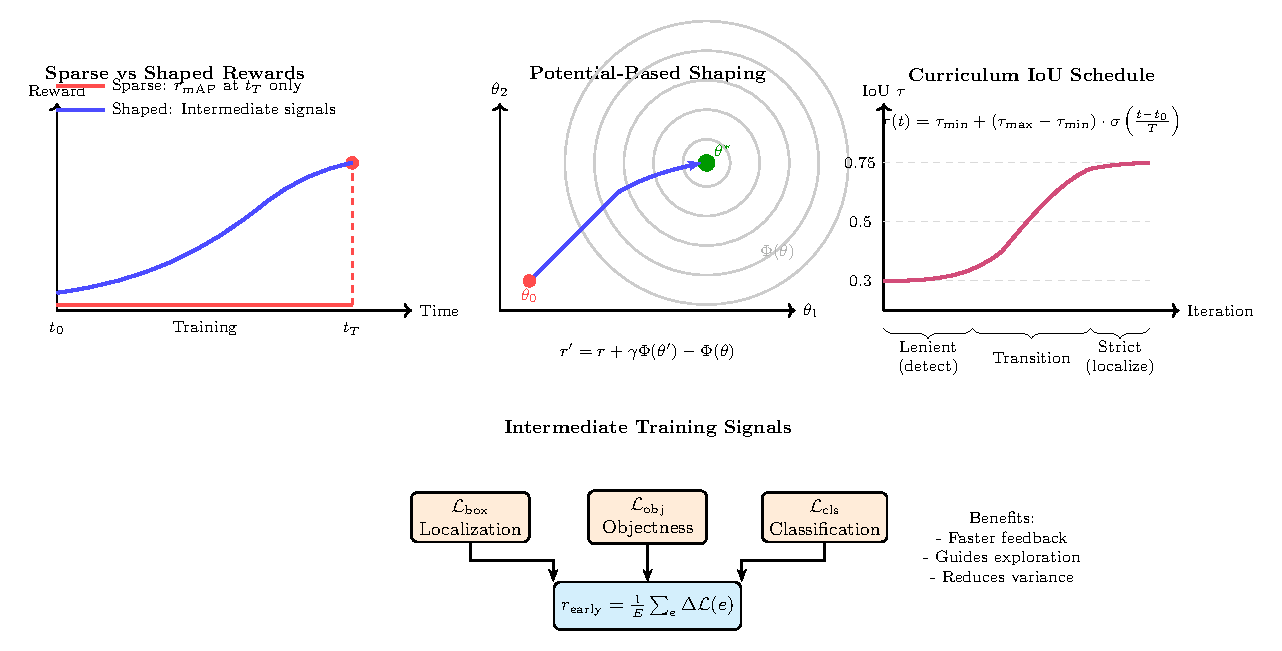
\includegraphics[width=\textwidth]{figures/ch07_fig2_reward_shaping.pdf}
\caption{Reward shaping strategies for synthetic data optimization. Top left: Comparison of sparse rewards (available only at training completion) versus shaped rewards (providing continuous feedback). Top center: Potential-based shaping guiding optimization toward known good configurations $\theta^*$. Top right: Curriculum IoU schedule transitioning from lenient detection thresholds to strict localization requirements. Bottom: Integration of intermediate training signals from YOLO loss components to provide early feedback.}
\label{fig:reward_shaping}
\end{figure}

\subsection{Multi-Objective Reward Balancing}

Synthetic data optimization involves multiple competing objectives: detection accuracy, computational efficiency, diversity, and domain alignment. Multi-objective reward balancing combines these signals into a coherent scalar reward while preserving sensitivity to each component.

Linear scalarization combines objectives with fixed weights:
\begin{equation}
r_{\text{linear}} = \sum_{i=1}^{M} w_i \cdot r_i
\label{eq:linear_scalarization}
\end{equation}

The choice of weights $\{w_i\}$ determines which points on the Pareto frontier are achievable through optimization. Different weight vectors trace out different regions of the frontier, but convex combinations cannot reach non-convex regions.

Chebyshev scalarization addresses this limitation by minimizing the maximum weighted deviation from an ideal point:
\begin{equation}
r_{\text{Chebyshev}} = -\max_{i \in \{1, \ldots, M\}} w_i \cdot |r_i^* - r_i|
\label{eq:chebyshev_scalarization}
\end{equation}
where $r_i^*$ represents the ideal (maximum achievable) value for objective $i$.

Achievement scalarizing functions generalize these approaches:
\begin{equation}
r_{\text{ASF}} = \min_{i} \frac{r_i - r_i^{\text{ref}}}{r_i^* - r_i^{\text{ref}}} + \rho \sum_{i} \frac{r_i - r_i^{\text{ref}}}{r_i^* - r_i^{\text{ref}}}
\label{eq:asf}
\end{equation}
where $r_i^{\text{ref}}$ is a reference point and $\rho > 0$ is a small constant ensuring strict monotonicity.

\begin{figure}[t]
\centering
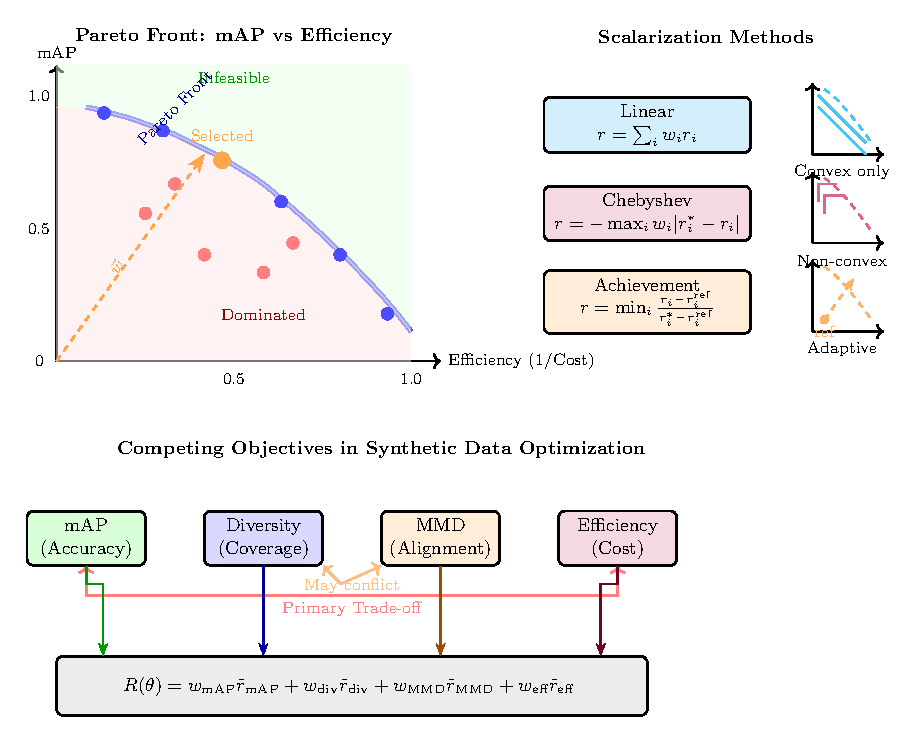
\includegraphics[width=\textwidth]{figures/ch07_fig3_pareto_front.pdf}
\caption{Multi-objective optimization in reward function design. Left: Pareto front illustrating the trade-off between mAP (accuracy) and efficiency, with dominated solutions shown in the shaded region and Pareto-optimal configurations on the frontier. A weight vector $\vec{w}$ determines which point on the frontier is selected. Right: Three scalarization methods (linear, Chebyshev, and achievement functions) with their geometric interpretations. Bottom: The competing objectives in synthetic data optimization and how they combine into the composite reward function.}
\label{fig:pareto_front}
\end{figure}

\subsection{Potential-Based Reward Shaping Theory}

The theoretical foundation for reward shaping rests on the concept of potential-based shaping, which guarantees that shaped rewards preserve optimal policies. Let $\Phi: \mathcal{S} \to \mathbb{R}$ be a potential function defined over states. The shaped reward is:
\begin{equation}
r'(s, a, s') = r(s, a, s') + \gamma \Phi(s') - \Phi(s)
\label{eq:potential_based_shaping}
\end{equation}
where $\gamma$ is the discount factor. This formulation ensures that policies optimal under $r'$ are also optimal under $r$, as the potential terms telescope when computing cumulative returns.

In the synthetic data optimization context, the state space consists of generator configurations $\theta$, and a natural potential function measures proximity to known good configurations:
\begin{equation}
\Phi(\theta) = \max_{\theta^* \in \Theta_{\text{good}}} \exp\left( -\frac{\|\theta - \theta^*\|^2}{2\sigma^2} \right)
\label{eq:configuration_potential}
\end{equation}
where $\Theta_{\text{good}}$ contains historically successful configurations.

The shaped reward encourages movement toward promising regions of the configuration space while preserving the global optimum defined by mAP:
\begin{equation}
r'(\theta, \theta') = r_{\text{mAP}}(\theta') + \gamma \Phi(\theta') - \Phi(\theta)
\label{eq:shaped_reward_synthetic}
\end{equation}

\section{Auxiliary Reward Components}
\label{sec:auxiliary_rewards}

Beyond the primary detection performance signal, auxiliary reward components address failure modes and desiderata that are not captured by mAP alone. These components include diversity bonuses that prevent mode collapse, domain alignment rewards that encourage distributional similarity to real data, intrinsic motivation signals that promote systematic exploration, and efficiency rewards that manage computational budgets.

\subsection{Diversity Bonuses}

Mode collapse, wherein the optimizer converges to generating highly similar synthetic images that exploit specific characteristics of the validation set, represents a significant failure mode in synthetic data optimization. Diversity bonuses explicitly reward variation in generated data, counteracting the tendency toward homogeneous outputs.

Let $\mathcal{D}_{\text{syn}}(\theta) = \{x_1, \ldots, x_n\}$ denote a batch of synthetic images generated with parameters $\theta$. The diversity bonus based on feature space coverage is:
\begin{equation}
r_{\text{diversity}} = \frac{1}{n(n-1)} \sum_{i \neq j} d(\phi(x_i), \phi(x_j))
\label{eq:diversity_bonus}
\end{equation}
where $\phi(\cdot)$ extracts features using a pretrained network and $d(\cdot, \cdot)$ is a distance metric in feature space.

Determinantal Point Processes (DPPs) provide a principled framework for measuring and encouraging diversity. The log-determinant of the feature kernel matrix serves as a diversity measure:
\begin{equation}
r_{\text{DPP}} = \log \det(K + \epsilon I)
\label{eq:dpp_diversity}
\end{equation}
where $K_{ij} = k(\phi(x_i), \phi(x_j))$ is a positive semi-definite kernel matrix and $\epsilon > 0$ ensures numerical stability.

Coverage metrics measure how well the synthetic data spans the feature space of real data:
\begin{equation}
r_{\text{coverage}} = \frac{1}{|\mathcal{D}_{\text{real}}|} \sum_{x \in \mathcal{D}_{\text{real}}} \mathbb{1}\left[ \min_{x' \in \mathcal{D}_{\text{syn}}} d(\phi(x), \phi(x')) < \epsilon \right]
\label{eq:coverage_reward}
\end{equation}

\subsection{Domain Alignment Rewards}

Domain alignment rewards encourage the synthetic data distribution to match the real data distribution, reducing the domain gap that degrades transfer performance. Maximum Mean Discrepancy (MMD) provides a kernel-based measure of distributional distance.

The empirical MMD between synthetic and real feature distributions is:
\begin{equation}
\widehat{\text{MMD}}^2 = \frac{1}{n^2} \sum_{i,j} k(z_i, z_j) + \frac{1}{m^2} \sum_{i,j} k(z'_i, z'_j) - \frac{2}{nm} \sum_{i,j} k(z_i, z'_j)
\label{eq:mmd}
\end{equation}
where $\{z_i\} = \{\phi(x_i)\}$ and $\{z'_i\} = \{\phi(x'_i)\}$ are feature representations of synthetic and real samples, respectively, and $k(\cdot, \cdot)$ is a characteristic kernel such as the Gaussian RBF kernel:
\begin{equation}
k(z, z') = \exp\left( -\frac{\|z - z'\|^2}{2\sigma^2} \right)
\label{eq:rbf_kernel}
\end{equation}

The domain alignment reward penalizes distributional discrepancy:
\begin{equation}
r_{\text{MMD}} = -\widehat{\text{MMD}}^2
\label{eq:mmd_reward}
\end{equation}

Fr\'{e}chet Inception Distance (FID) provides an alternative distributional measure based on Gaussian approximations:
\begin{equation}
\text{FID} = \|\mu_{\text{syn}} - \mu_{\text{real}}\|^2 + \text{Tr}\left( \Sigma_{\text{syn}} + \Sigma_{\text{real}} - 2(\Sigma_{\text{syn}} \Sigma_{\text{real}})^{1/2} \right)
\label{eq:fid}
\end{equation}
where $(\mu_{\text{syn}}, \Sigma_{\text{syn}})$ and $(\mu_{\text{real}}, \Sigma_{\text{real}})$ are the mean and covariance of feature distributions.

Domain confusion rewards leverage domain discriminator networks trained to distinguish synthetic from real images. The reward encourages synthetic data that fools the discriminator:
\begin{equation}
r_{\text{confusion}} = -\mathbb{E}_{x \sim \mathcal{D}_{\text{syn}}} \left[ \log D(x) \right]
\label{eq:domain_confusion}
\end{equation}
where $D(x)$ outputs the probability that $x$ is synthetic.

\subsection{Intrinsic Motivation}

Intrinsic motivation provides reward signals that encourage exploration of the parameter space independent of task-specific performance. These signals address the exploration-exploitation trade-off by rewarding the agent for visiting novel configurations.

Random Network Distillation (RND) measures novelty by comparing the output of a randomly initialized network $f_{\text{random}}$ with a learned predictor $f_{\text{pred}}$:
\begin{equation}
r_{\text{RND}}(\theta) = \|f_{\text{pred}}(\theta) - f_{\text{random}}(\theta)\|^2
\label{eq:rnd_reward}
\end{equation}

The predictor is trained to match the random network's outputs on visited configurations, so high prediction error indicates novelty.

Curiosity-driven exploration rewards visiting states that are difficult to predict:
\begin{equation}
r_{\text{curiosity}}(\theta, \theta') = \|g_{\text{pred}}(\theta, a) - \phi(\theta')\|^2
\label{eq:curiosity_reward}
\end{equation}
where $g_{\text{pred}}$ attempts to predict the feature representation of the next state given the current state and action, and $\phi(\cdot)$ is a learned state encoder.

Count-based exploration bonuses reward visiting infrequently-seen configurations:
\begin{equation}
r_{\text{count}}(\theta) = \frac{\beta}{\sqrt{N(\theta) + 1}}
\label{eq:count_bonus}
\end{equation}
where $N(\theta)$ counts visits to configuration $\theta$ (or a discretized approximation thereof) and $\beta$ scales the bonus magnitude.

\subsection{Exploration Bonuses}

Structured exploration bonuses encourage systematic coverage of the parameter space, preventing premature convergence to local optima. These bonuses complement intrinsic motivation by incorporating prior knowledge about promising exploration directions.

Boundary exploration rewards visiting configurations near the edges of the parameter space:
\begin{equation}
r_{\text{boundary}}(\theta) = \max_i \left( \max(0, \theta_i - \theta_i^{\text{hi}} + \epsilon) + \max(0, \theta_i^{\text{lo}} - \theta_i + \epsilon) \right)
\label{eq:boundary_exploration}
\end{equation}

Parameter-specific exploration bonuses can emphasize under-explored dimensions:
\begin{equation}
r_{\text{dim-explore}}(\theta) = \sum_i \frac{w_i}{\text{Var}(\theta_i^{(1:t)}) + \epsilon}
\label{eq:dim_exploration}
\end{equation}
where $\text{Var}(\theta_i^{(1:t)})$ is the empirical variance of dimension $i$ across visited configurations and $w_i$ weights the importance of exploring each dimension.

\subsection{Efficiency and Budget Rewards}

Practical synthetic data optimization operates under computational budget constraints, necessitating rewards that balance performance against resource consumption.

Training efficiency rewards favor configurations that yield good performance with minimal training:
\begin{equation}
r_{\text{efficiency}} = \frac{\text{mAP}(\theta)}{E_{\text{convergence}}(\theta)}
\label{eq:efficiency_reward}
\end{equation}
where $E_{\text{convergence}}(\theta)$ measures the number of epochs required to reach convergence.

Data efficiency rewards prefer configurations requiring smaller synthetic datasets:
\begin{equation}
r_{\text{data-eff}} = \text{mAP}(\theta) - \lambda \cdot \log(|\mathcal{D}_{\text{syn}}(\theta)|)
\label{eq:data_efficiency}
\end{equation}

Computational cost penalties discourage expensive configurations:
\begin{equation}
r_{\text{cost}} = -\lambda_{\text{cost}} \cdot \text{Cost}(\theta)
\label{eq:cost_penalty}
\end{equation}
where $\text{Cost}(\theta)$ may include rendering time, storage requirements, and training compute.

\section{The Composite Reward Function}
\label{sec:composite_reward}

The individual reward components developed in preceding sections must be integrated into a coherent composite reward function that balances competing objectives, maintains appropriate scaling, and provides stable learning signals. This section presents the complete mathematical formulation, discusses weight balancing strategies, and develops normalization and smoothing techniques essential for practical implementation.

\subsection{Complete Formulation}

The composite reward function integrates primary detection metrics, statistical reliability adjustments, auxiliary signals, and efficiency considerations:
\begin{equation}
\begin{aligned}
R(\theta) = \; & w_{\text{mAP}} \cdot \tilde{r}_{\text{mAP}}(\theta) \\
& + w_{\text{conf}} \cdot \tilde{r}_{\text{confidence}}(\theta) \\
& + w_{\text{div}} \cdot \tilde{r}_{\text{diversity}}(\theta) \\
& + w_{\text{MMD}} \cdot \tilde{r}_{\text{MMD}}(\theta) \\
& + w_{\text{explore}} \cdot \tilde{r}_{\text{exploration}}(\theta) \\
& + w_{\text{eff}} \cdot \tilde{r}_{\text{efficiency}}(\theta) \\
& + w_{\text{shape}} \cdot F(\theta, \theta')
\end{aligned}
\label{eq:composite_reward}
\end{equation}
where tildes denote normalized reward components and $F(\theta, \theta')$ represents the potential-based shaping term.

The conservative mAP component incorporates bootstrap uncertainty:
\begin{equation}
\tilde{r}_{\text{mAP}}(\theta) = \frac{\widehat{\text{mAP}}(\theta) - \kappa \cdot \hat{\sigma}_{\text{boot}}(\theta) - \mu_{\text{mAP}}}{\sigma_{\text{mAP}}}
\label{eq:normalized_map}
\end{equation}
where $\mu_{\text{mAP}}$ and $\sigma_{\text{mAP}}$ are running estimates of the mean and standard deviation of mAP values across the optimization history.

\begin{figure}[t]
\centering
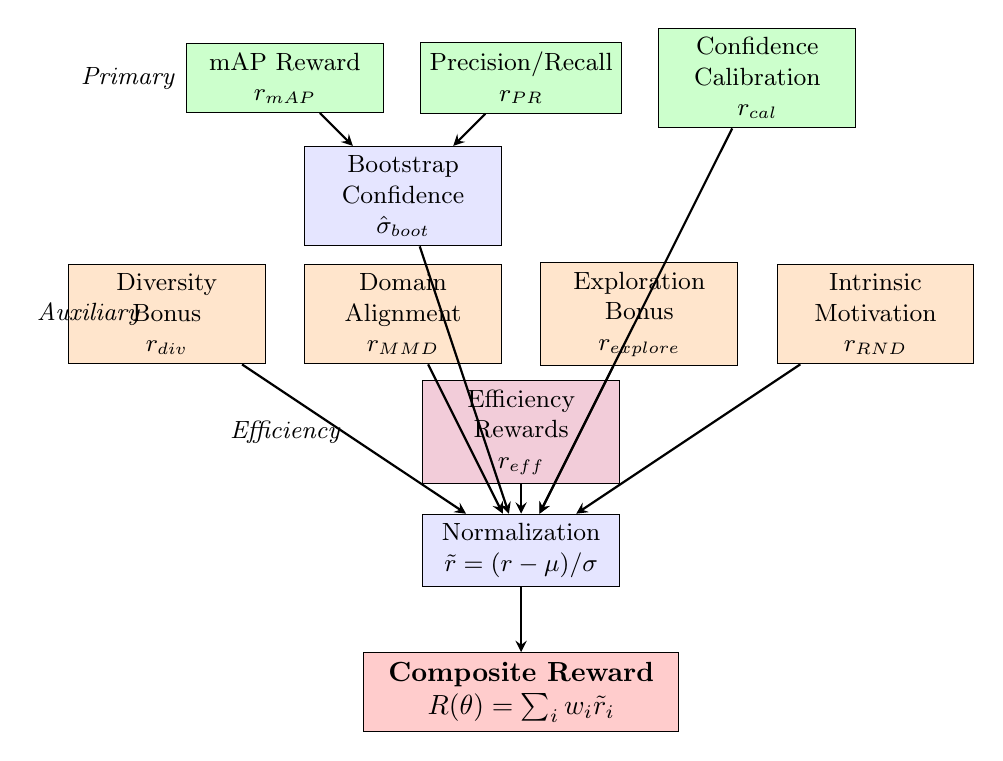
\begin{tikzpicture}[
    node distance=1.5cm,
    component/.style={rectangle, draw=black, fill=blue!10, minimum width=2.5cm, minimum height=0.8cm, align=center, font=\small},
    primary/.style={rectangle, draw=black, fill=green!20, minimum width=2.5cm, minimum height=0.8cm, align=center, font=\small},
    auxiliary/.style={rectangle, draw=black, fill=orange!20, minimum width=2.5cm, minimum height=0.8cm, align=center, font=\small},
    efficiency/.style={rectangle, draw=black, fill=purple!20, minimum width=2.5cm, minimum height=0.8cm, align=center, font=\small},
    composite/.style={rectangle, draw=black, fill=red!20, minimum width=4cm, minimum height=1cm, align=center, font=\normalsize\bfseries},
    arrow/.style={->, thick, >=stealth}
]

% Primary rewards
\node[primary] (map) at (0, 4) {mAP Reward\\$r_{\text{mAP}}$};
\node[primary] (prec) at (3, 4) {Precision/Recall\\$r_{\text{PR}}$};
\node[primary] (conf) at (6, 4) {Confidence\\Calibration\\$r_{\text{cal}}$};

% Statistical adjustment
\node[component] (bootstrap) at (1.5, 2.5) {Bootstrap\\Confidence\\$\hat{\sigma}_{\text{boot}}$};

% Auxiliary rewards
\node[auxiliary] (div) at (-1.5, 1) {Diversity\\Bonus\\$r_{\text{div}}$};
\node[auxiliary] (mmd) at (1.5, 1) {Domain\\Alignment\\$r_{\text{MMD}}$};
\node[auxiliary] (explore) at (4.5, 1) {Exploration\\Bonus\\$r_{\text{explore}}$};
\node[auxiliary] (intrinsic) at (7.5, 1) {Intrinsic\\Motivation\\$r_{\text{RND}}$};

% Efficiency rewards
\node[efficiency] (eff) at (3, -0.5) {Efficiency\\Rewards\\$r_{\text{eff}}$};

% Normalization
\node[component] (norm) at (3, -2) {Normalization\\$\tilde{r} = (r - \mu)/\sigma$};

% Composite reward
\node[composite] (composite) at (3, -3.8) {Composite Reward\\$R(\theta) = \sum_i w_i \tilde{r}_i$};

% Arrows
\draw[arrow] (map) -- (bootstrap);
\draw[arrow] (prec) -- (bootstrap);
\draw[arrow] (conf) -- (norm);
\draw[arrow] (bootstrap) -- (norm);
\draw[arrow] (div) -- (norm);
\draw[arrow] (mmd) -- (norm);
\draw[arrow] (explore) -- (norm);
\draw[arrow] (intrinsic) -- (norm);
\draw[arrow] (eff) -- (norm);
\draw[arrow] (norm) -- (composite);

% Labels
\node[font=\small\itshape] at (-2, 4) {Primary};
\node[font=\small\itshape] at (-2.5, 1) {Auxiliary};
\node[font=\small\itshape] at (0, -0.5) {Efficiency};

\end{tikzpicture}
\caption{Architecture of the composite reward function showing the flow from primary detection metrics through statistical adjustment and normalization to the final composite reward. Primary components (green) capture detection performance, auxiliary components (orange) encourage exploration and domain alignment, and efficiency components (purple) manage computational resources.}
\label{fig:reward_architecture}
\end{figure}

\subsection{Weight Balancing Strategies}

The selection of component weights $\{w_i\}$ profoundly influences optimization dynamics and final performance. Several strategies inform weight selection.

Scale-based weighting sets weights inversely proportional to the typical magnitude of each component, ensuring roughly equal contribution to the composite reward:
\begin{equation}
w_i \propto \frac{1}{\text{Var}(r_i)^{1/2}}
\label{eq:scale_based_weights}
\end{equation}

Importance-based weighting reflects the relative priority of different objectives, typically placing highest weight on the primary mAP signal:
\begin{equation}
w_{\text{mAP}} : w_{\text{auxiliary}} : w_{\text{explore}} = 10 : 3 : 1
\label{eq:importance_weights}
\end{equation}

Adaptive weighting adjusts weights during optimization to maintain balance as the relative variability of components changes:
\begin{equation}
w_i(t) = \frac{\alpha_i / \hat{\sigma}_i(t)}{\sum_j \alpha_j / \hat{\sigma}_j(t)}
\label{eq:adaptive_weights}
\end{equation}
where $\alpha_i$ encodes prior importance and $\hat{\sigma}_i(t)$ is the running standard deviation of component $i$.

\begin{table}[t]
\centering
\caption{Recommended reward component weights and their effects on optimization behavior. The weight ranges reflect typical values that balance effectiveness against potential negative side effects.}
\label{tab:reward_weights}
\begin{tabular}{p{2.5cm}p{2cm}p{2.5cm}p{5cm}}
\toprule
\textbf{Component} & \textbf{Weight Range} & \textbf{Primary Effect} & \textbf{Considerations} \\
\midrule
$w_{\text{mAP}}$ & $0.5$--$0.8$ & Detection accuracy & Dominant signal; higher values accelerate convergence but may cause overfitting to validation set \\
\addlinespace
$w_{\text{conf}}$ & $0.05$--$0.15$ & Calibration quality & Improves reliability of confidence scores; essential for threshold-based deployment \\
\addlinespace
$w_{\text{div}}$ & $0.05$--$0.2$ & Prevents mode collapse & Higher values encourage diversity at potential cost to peak performance \\
\addlinespace
$w_{\text{MMD}}$ & $0.1$--$0.25$ & Domain alignment & Critical for sim-to-real transfer; excessive weight may over-constrain generator \\
\addlinespace
$w_{\text{explore}}$ & $0.02$--$0.1$ & Exploration breadth & Decays during optimization; prevents premature convergence \\
\addlinespace
$w_{\text{eff}}$ & $0.05$--$0.15$ & Computational cost & Important under budget constraints; may sacrifice peak performance \\
\addlinespace
$w_{\text{shape}}$ & $0.05$--$0.1$ & Learning speed & Guides early exploration; should not dominate terminal behavior \\
\bottomrule
\end{tabular}
\end{table}

\subsection{Normalization Techniques}

Reward normalization ensures that different components contribute appropriately to the composite signal and that the reward scale remains stable throughout optimization.

Z-score normalization transforms each component to zero mean and unit variance:
\begin{equation}
\tilde{r}_i = \frac{r_i - \mu_i}{\sigma_i + \epsilon}
\label{eq:zscore_normalization}
\end{equation}
where $\mu_i$ and $\sigma_i$ are computed using exponential moving averages to adapt to non-stationary reward distributions.

The running statistics are updated as:
\begin{equation}
\mu_i(t) = \beta \mu_i(t-1) + (1-\beta) r_i(t), \quad \sigma_i^2(t) = \beta \sigma_i^2(t-1) + (1-\beta) (r_i(t) - \mu_i(t))^2
\label{eq:running_statistics}
\end{equation}
where $\beta \in [0.9, 0.999]$ controls the adaptation rate.

Min-max normalization bounds rewards to a fixed interval $[0, 1]$:
\begin{equation}
\tilde{r}_i = \frac{r_i - r_i^{\min}}{r_i^{\max} - r_i^{\min} + \epsilon}
\label{eq:minmax_normalization}
\end{equation}

Percentile-based normalization provides robustness to outliers:
\begin{equation}
\tilde{r}_i = \frac{r_i - Q_{0.05}(r_i)}{Q_{0.95}(r_i) - Q_{0.05}(r_i) + \epsilon}
\label{eq:percentile_normalization}
\end{equation}
where $Q_p(r_i)$ denotes the $p$-th percentile of the historical distribution of $r_i$.

\subsection{Temporal Smoothing}

Temporal smoothing reduces the impact of noisy reward estimates by averaging over recent history. Exponential Moving Average (EMA) smoothing is particularly effective:
\begin{equation}
R_{\text{EMA}}(t) = \alpha R(t) + (1 - \alpha) R_{\text{EMA}}(t-1)
\label{eq:ema_smoothing}
\end{equation}
where $\alpha \in [0.1, 0.3]$ balances responsiveness against noise reduction.

The effective window size of EMA smoothing is approximately $1/\alpha$, so $\alpha = 0.2$ corresponds to averaging over approximately five recent observations.

Multi-scale temporal smoothing combines estimates at different time scales:
\begin{equation}
R_{\text{multi}}(t) = \sum_{k=1}^{K} \gamma_k R_{\text{EMA}}^{(k)}(t)
\label{eq:multiscale_smoothing}
\end{equation}
where $R_{\text{EMA}}^{(k)}$ uses smoothing parameter $\alpha_k$ and $\sum_k \gamma_k = 1$.

\subsection{Complete Reward Computation Algorithm}

Algorithm~\ref{alg:complete_reward} presents the complete procedure for computing the composite reward given a generator configuration, integrating all components discussed in this chapter.

\begin{algorithm}[t]
\caption{Complete Composite Reward Computation}
\label{alg:complete_reward}
\begin{algorithmic}[1]
\Require Generator configuration $\theta$, validation set $\mathcal{D}_{\text{val}}$, real data features $\mathcal{F}_{\text{real}}$
\Require Historical statistics $\mathcal{H} = \{\mu_i, \sigma_i, R_{\text{EMA}}\}$, component weights $\{w_i\}$
\Require Hyperparameters: $B$ (bootstrap samples), $\kappa$ (conservatism), $\alpha$ (EMA rate)
\Ensure Composite reward $R$, updated statistics $\mathcal{H}'$
\State \textbf{Generate synthetic data and train detector:}
\State $\mathcal{D}_{\text{syn}} \gets \text{Generate}(\theta)$
\State $f_\phi \gets \text{TrainYOLO}(\mathcal{D}_{\text{syn}})$
\State
\State \textbf{Compute primary reward with bootstrap confidence:}
\State $\widehat{\text{mAP}}, \hat{\sigma}_{\text{boot}} \gets \text{BootstrapCI}(\mathcal{D}_{\text{val}}, f_\phi, B)$ \Comment{Algorithm~\ref{alg:bootstrap_confidence}}
\State $r_{\text{mAP}} \gets \widehat{\text{mAP}} - \kappa \cdot \hat{\sigma}_{\text{boot}}$
\State
\State \textbf{Compute auxiliary rewards:}
\State $\mathcal{F}_{\text{syn}} \gets \text{ExtractFeatures}(\mathcal{D}_{\text{syn}})$
\State $r_{\text{MMD}} \gets -\text{MMD}^2(\mathcal{F}_{\text{syn}}, \mathcal{F}_{\text{real}})$
\State $r_{\text{div}} \gets \text{DiversityScore}(\mathcal{F}_{\text{syn}})$
\State $r_{\text{explore}} \gets \text{ExplorationBonus}(\theta, \mathcal{H})$
\State $r_{\text{eff}} \gets -\lambda_{\text{cost}} \cdot \text{TrainingCost}$
\State
\State \textbf{Normalize all components:}
\For{$i \in \{\text{mAP}, \text{MMD}, \text{div}, \text{explore}, \text{eff}\}$}
    \State $\tilde{r}_i \gets (r_i - \mu_i) / (\sigma_i + \epsilon)$
    \State $\mu_i \gets \beta \mu_i + (1-\beta) r_i$ \Comment{Update running mean}
    \State $\sigma_i^2 \gets \beta \sigma_i^2 + (1-\beta)(r_i - \mu_i)^2$ \Comment{Update running variance}
\EndFor
\State
\State \textbf{Compute composite reward:}
\State $R_{\text{raw}} \gets w_{\text{mAP}} \tilde{r}_{\text{mAP}} + w_{\text{MMD}} \tilde{r}_{\text{MMD}} + w_{\text{div}} \tilde{r}_{\text{div}} + w_{\text{explore}} \tilde{r}_{\text{explore}} + w_{\text{eff}} \tilde{r}_{\text{eff}}$
\State
\State \textbf{Apply temporal smoothing:}
\State $R \gets \alpha R_{\text{raw}} + (1-\alpha) R_{\text{EMA}}$
\State $R_{\text{EMA}} \gets R$
\State
\State \Return $R$, $\mathcal{H}' = \{\mu_i, \sigma_i, R_{\text{EMA}}\}$
\end{algorithmic}
\end{algorithm}

\section{Reward Function Pitfalls}
\label{sec:pitfalls}

The design of reward functions for synthetic data optimization presents numerous opportunities for failure. This section catalogs common pitfalls, develops diagnostic techniques for their detection, and presents mitigation strategies that have proven effective in practice.

\subsection{Reward Hacking in Synthetic Data Generation}

Reward hacking occurs when the optimizer discovers configurations that achieve high reward through mechanisms other than the intended improvement in detector quality. In synthetic data generation, reward hacking manifests through several characteristic patterns.

Validation set memorization occurs when the generator discovers specific visual patterns present in validation images and produces synthetic data biased toward these patterns. The resulting detector achieves high validation mAP by exploiting correlations specific to the validation set rather than learning generalizable detection capabilities. Detection involves monitoring the gap between validation and held-out test performance:
\begin{equation}
\Delta_{\text{overfit}} = \text{mAP}_{\text{val}} - \text{mAP}_{\text{test}}
\label{eq:overfit_gap}
\end{equation}

When $\Delta_{\text{overfit}}$ exceeds a threshold (typically 0.05), validation set memorization is likely occurring.

Metric gaming exploits characteristics of the mAP computation itself. The mAP metric provides minimal penalties for excessive false-positive boxes, allowing generators to produce synthetic data that trains detectors to output many redundant predictions. This artificially inflates AP scores without improving actual detection quality. Detection requires monitoring prediction count statistics:
\begin{equation}
\bar{N}_{\text{pred}} = \frac{1}{|\mathcal{D}_{\text{val}}|} \sum_{x \in \mathcal{D}_{\text{val}}} |\hat{\mathcal{Y}}(x)|
\label{eq:prediction_count}
\end{equation}

Abnormally high $\bar{N}_{\text{pred}}$ relative to ground truth object counts indicates metric gaming.

Trivial solutions represent degenerate configurations that achieve reward through collapse to simple but useless patterns. Examples include generators that produce near-constant images, resulting in detectors that output fixed predictions regardless of input. Detection monitors feature diversity:
\begin{equation}
\text{Diversity} = \text{Var}(\phi(\mathcal{D}_{\text{syn}}))
\label{eq:feature_diversity}
\end{equation}

Collapse is indicated when diversity falls below a threshold determined from healthy configurations.

\subsection{Degenerate Solutions and Detection}

Beyond reward hacking, optimization may converge to degenerate solutions that fail to satisfy implicit constraints not captured by the reward function.

Mode collapse produces synthetic data concentrated in a small region of the possible image space, failing to cover the diversity present in real-world scenarios. The diversity bonus discussed in Section~\ref{sec:auxiliary_rewards} provides direct mitigation, but detection requires ongoing monitoring:
\begin{equation}
\text{Coverage}(t) = \frac{|\{x \in \mathcal{D}_{\text{real}} : \exists x' \in \mathcal{D}_{\text{syn}}(t), d(\phi(x), \phi(x')) < \epsilon\}|}{|\mathcal{D}_{\text{real}}|}
\label{eq:coverage_metric}
\end{equation}

Declining coverage over optimization iterations indicates progressive mode collapse.

Parameter space collapse occurs when the optimizer converges to a narrow region of the parameter space, failing to explore potentially superior configurations. This manifests as decreasing variance in the visited configurations:
\begin{equation}
\text{Var}_\theta(t) = \frac{1}{d} \sum_{i=1}^{d} \text{Var}(\theta_i^{(t-W:t)})
\label{eq:parameter_variance}
\end{equation}
where the variance is computed over a sliding window of $W$ recent configurations.

Detection requires comparing $\text{Var}_\theta(t)$ against expected values given the optimization algorithm and iteration count.

\begin{figure}[t]
\centering
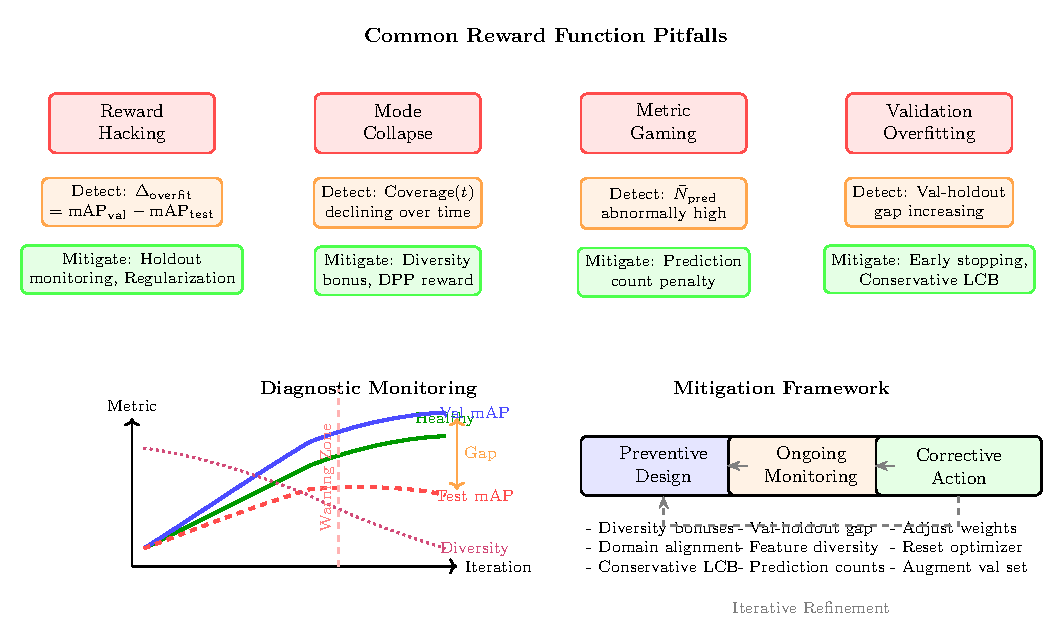
\includegraphics[width=\textwidth]{figures/ch07_fig4_pitfalls.pdf}
\caption{Common reward function pitfalls and mitigation strategies. Top: Four major pitfalls (reward hacking, mode collapse, metric gaming, and validation overfitting) with their detection metrics and mitigation approaches. Bottom left: Diagnostic monitoring showing the divergence between validation mAP (potentially overfitting) and test mAP, along with declining diversity indicating mode collapse. Bottom right: Three-phase mitigation framework combining preventive design, ongoing monitoring, and corrective action in an iterative refinement loop.}
\label{fig:pitfalls}
\end{figure}

\subsection{Overfitting to Validation Set}

The small validation sets typical of synthetic data optimization scenarios create severe overfitting risk. Configurations that achieve high validation reward may exploit idiosyncrasies of the specific validation images rather than learning generally transferable generation strategies.

Holdout monitoring reserves a portion of available real images as a test set never used for reward computation:
\begin{equation}
\text{mAP}_{\text{holdout}}(\theta) = \text{mAP}(\mathcal{D}_{\text{holdout}}, f_{\phi(\theta)})
\label{eq:holdout_map}
\end{equation}

Periodic evaluation on the holdout set (without using results for optimization) enables detection of validation overfitting.

Regularization through reward penalty terms discourages configurations that deviate excessively from prior knowledge:
\begin{equation}
r_{\text{regularized}} = r_{\text{mAP}} - \lambda_{\text{reg}} \|\theta - \theta_0\|^2
\label{eq:regularization}
\end{equation}
where $\theta_0$ represents a default or previously successful configuration.

Early stopping terminates optimization when validation performance plateaus while auxiliary metrics suggest declining quality:
\begin{equation}
\text{Stop if } \frac{d\text{mAP}_{\text{val}}}{dt} < \epsilon_{\text{stop}} \text{ and } \frac{d\text{Diversity}}{dt} < 0
\label{eq:early_stopping}
\end{equation}

\subsection{Shortcut Learning}

Shortcut learning occurs when detectors trained on synthetic data learn to exploit superficial correlations rather than semantically meaningful features. Common shortcuts include background texture correlations, object-background co-occurrence patterns, and rendering artifacts that distinguish synthetic from real images.

Diagnostic evaluation requires probing detector behavior under controlled perturbations. Background randomization tests whether the detector relies on background features:
\begin{equation}
\Delta_{\text{bg}} = \text{mAP}(\mathcal{D}_{\text{original}}) - \text{mAP}(\mathcal{D}_{\text{bg-random}})
\label{eq:background_sensitivity}
\end{equation}

Large $\Delta_{\text{bg}}$ indicates problematic background dependence.

Object-only evaluation tests detector performance on images with objects isolated from their original backgrounds, revealing whether the detector has learned object-intrinsic features or relies on contextual cues.

Mitigation strategies include aggressive background domain randomization in the synthetic data generator, explicit penalties for background sensitivity in the reward function, and multi-environment training that exposes detectors to varied contexts for the same objects.

\subsection{Mitigation Strategy Summary}

Effective mitigation of reward function pitfalls requires a multi-pronged approach combining preventive design, ongoing monitoring, and corrective interventions.

Preventive design incorporates diversity bonuses, domain alignment rewards, and conservative reward estimation from the outset, reducing the optimizer's ability to exploit reward function weaknesses.

Ongoing monitoring tracks diagnostic metrics including the validation-holdout gap, prediction count statistics, feature diversity, and parameter space variance. Automated alerts trigger when metrics exceed thresholds indicative of pathological behavior.

Corrective interventions include reward function adjustment (increasing diversity or exploration weights), optimizer reset to diverse initial conditions, and augmentation of the validation set when possible.

\section{Implementation Considerations}
\label{sec:implementation}

The translation of mathematical reward formulations into practical implementations requires attention to numerical stability, computational efficiency, and integration with existing machine learning infrastructure. This section addresses key implementation considerations that ensure reliable reward computation in production systems.

\subsection{Reward Normalization}

Effective reward normalization requires careful initialization and adaptation strategies to handle the non-stationary reward distributions encountered during optimization.

Burn-in initialization collects reward statistics during an initial exploration phase before applying normalization:
\begin{equation}
\mu_i^{(0)} = \frac{1}{T_{\text{burn}}} \sum_{t=1}^{T_{\text{burn}}} r_i(t), \quad \sigma_i^{(0)} = \sqrt{\frac{1}{T_{\text{burn}}-1} \sum_{t=1}^{T_{\text{burn}}} (r_i(t) - \mu_i^{(0)})^2}
\label{eq:burnin_initialization}
\end{equation}

During the burn-in period, unnormalized rewards are used, accepting higher variance in exchange for accurate initialization.

Adaptation rate scheduling adjusts the EMA parameter $\beta$ over time, using faster adaptation early (lower $\beta$) and slower adaptation later (higher $\beta$):
\begin{equation}
\beta(t) = \beta_{\text{final}} - (\beta_{\text{final}} - \beta_{\text{init}}) \exp(-t / \tau_\beta)
\label{eq:beta_schedule}
\end{equation}

Per-component normalization applies different strategies to different reward components based on their distributional characteristics. Bounded components (e.g., mAP $\in [0,1]$) may use min-max normalization, while unbounded components (e.g., MMD distances) require z-score normalization.

\subsection{Value Baseline for Variance Reduction}

When using policy gradient methods for optimization, a learned value baseline reduces gradient variance while maintaining unbiased gradient estimates. The baseline $V(s)$ estimates expected future reward from state $s$.

The advantage function quantifies how much better an action is relative to the baseline expectation:
\begin{equation}
A(s, a) = R(s, a) - V(s)
\label{eq:advantage}
\end{equation}

Using advantages rather than raw rewards in policy gradient updates substantially reduces variance:
\begin{equation}
\nabla_\theta J(\theta) = \mathbb{E}\left[ A(s, a) \nabla_\theta \log \pi_\theta(a|s) \right]
\label{eq:advantage_gradient}
\end{equation}

The value function can be parameterized as a neural network $V_\psi(s)$ trained to minimize temporal difference error:
\begin{equation}
\mathcal{L}_V(\psi) = \mathbb{E}\left[ (R(s, a) + \gamma V_\psi(s') - V_\psi(s))^2 \right]
\label{eq:value_loss}
\end{equation}

In synthetic data optimization, the state representation may include summary statistics of recent configurations, historical performance metrics, and remaining budget information.

\subsection{Clipping and Scaling}

Reward clipping prevents extreme values from destabilizing learning, while scaling ensures appropriate gradient magnitudes.

Hard clipping bounds rewards to a fixed interval:
\begin{equation}
R_{\text{clipped}} = \max(\min(R, R_{\text{max}}), R_{\text{min}})
\label{eq:hard_clipping}
\end{equation}

Typical bounds are $R_{\text{min}} = -10$ and $R_{\text{max}} = 10$ after normalization.

Soft clipping using tanh provides smoother gradients near boundaries:
\begin{equation}
R_{\text{soft}} = R_{\text{max}} \cdot \tanh(R / R_{\text{max}})
\label{eq:soft_clipping}
\end{equation}

Huber-style clipping combines linear behavior near zero with bounded growth at extremes:
\begin{equation}
R_{\text{Huber}} = \begin{cases}
R & \text{if } |R| \leq \delta \\
\delta \cdot \text{sign}(R) \cdot (1 + \log(|R|/\delta)) & \text{otherwise}
\end{cases}
\label{eq:huber_clipping}
\end{equation}

Scale adjustment ensures that the effective learning rate remains appropriate as reward statistics evolve:
\begin{equation}
R_{\text{scaled}} = R / \max(\sigma_R, \sigma_{\text{min}})
\label{eq:scale_adjustment}
\end{equation}
where $\sigma_{\text{min}}$ prevents division by near-zero values.

\subsection{Numerical Stability}

Numerical stability requires careful handling of edge cases, appropriate precision, and defensive programming practices.

Division safety prevents division by zero or near-zero values:
\begin{equation}
\frac{a}{b} \to \frac{a}{b + \epsilon \cdot \text{sign}(b)}
\label{eq:safe_division}
\end{equation}
where $\epsilon = 10^{-8}$ is typical for float32 precision.

Logarithm safety handles arguments near zero:
\begin{equation}
\log(x) \to \log(\max(x, \epsilon))
\label{eq:safe_log}
\end{equation}

Exponential overflow prevention clips arguments before exponentiation:
\begin{equation}
\exp(x) \to \exp(\min(x, 80))
\label{eq:safe_exp}
\end{equation}

For softmax operations, the log-sum-exp trick maintains precision:
\begin{equation}
\log \sum_i \exp(x_i) = x_{\max} + \log \sum_i \exp(x_i - x_{\max})
\label{eq:logsumexp}
\end{equation}

Mixed precision considerations arise when using float16 for efficiency. Reward computations should generally use float32 to maintain precision, with conversion only for final storage or communication.

Gradient checkpointing for long-horizon reward computation trades memory for computation, recomputing intermediate values during backpropagation rather than storing them. This is particularly relevant when reward computation involves backpropagation through the detector training process.

\section{Chapter Summary}

This chapter has developed a comprehensive framework for reward function engineering in the context of synthetic data optimization for object detection. The presentation began with the mathematical formulation of mean Average Precision and its component metrics, establishing the primary reward signal that guides optimization toward improved detector performance. The treatment of small validation sets introduced bootstrap confidence estimation and cross-validation strategies that address the statistical challenges inherent in scenarios with limited real-world imagery, providing principled approaches to variance reduction and conservative reward estimation.

The discussion of reward shaping strategies developed intermediate reward signals based on training dynamics, curriculum-based schedules that progressively increase evaluation stringency, and multi-objective balancing techniques that integrate competing objectives. The theoretical foundation of potential-based reward shaping ensures that shaped rewards preserve optimal policies while accelerating learning.

Auxiliary reward components address failure modes not captured by detection metrics alone, including diversity bonuses that prevent mode collapse, domain alignment rewards based on Maximum Mean Discrepancy that encourage distributional similarity to real data, and intrinsic motivation signals that promote systematic exploration of the parameter space. Efficiency rewards manage computational budgets while maintaining focus on detection quality.

The complete composite reward formulation integrates all components with appropriate normalization and temporal smoothing, providing stable learning signals throughout optimization. The analysis of reward function pitfalls cataloged common failure modes including reward hacking, mode collapse, and validation set overfitting, along with detection techniques and mitigation strategies.

Implementation considerations addressed the practical challenges of reward normalization, value baseline construction for variance reduction, clipping and scaling strategies, and numerical stability requirements. The algorithms and mathematical formulations presented provide a complete specification for implementing robust reward computation in production synthetic data optimization systems.

The reward function engineering principles developed in this chapter provide the foundation for effective reinforcement learning optimization of synthetic data generation parameters. When properly implemented, the composite reward function enables discovery of generator configurations that yield detectors achieving superior real-world performance while maintaining robustness against the pathological behaviors that can arise when optimizing complex, high-dimensional systems under limited supervision.
